\documentclass[12pt,twoside]{report}
\usepackage[a4paper,width=150mm,headheight=110pt,top=25mm,bottom=25mm]{geometry}
\usepackage[utf8]{inputenc}
\usepackage{listings}
\usepackage{graphicx}
\usepackage{tikz}
\usepackage{pgffor} 
\usepackage{float}
\usepackage{graphics} 
\usepackage{fancyhdr}
\usepackage[round, numbers,authoryear]{natbib}
\usepackage{color}
\usepackage{indentfirst}

\graphicspath{{images/}}

\definecolor{mycolor}{RGB}{30,75,180}
\definecolor{mycolor2}{RGB}{40,75,90}
\definecolor{red}{RGB}{200,0,0}
\usepackage[colorlinks = true,
            linkcolor = mycolor,
            urlcolor  = mycolor,
            citecolor = mycolor,
            anchorcolor = mycolor]{hyperref}

\usepackage[hypcap=true,font={small,it}]{caption}
\usetikzlibrary{calc}

\captionsetup{belowskip=2pt,aboveskip=2pt}
\bibliographystyle{abbrvnat}

\renewcommand{\chaptername}{}

\renewcommand{\figureautorefname}{figure} % lower case default ref
\renewcommand{\tableautorefname}{table} % lower case default ref
\newcommand{\latex}{\LaTeX\xspace}
\newcommand{\mcite}[1]{\textcolor{mycolor}{\citeauthor{#1} (\citeyear{#1})}}
\newcommand{\hcite}[1]{(\textcolor{mycolor}{\citeauthor{#1}, \citeyear{#1}})}
\newcommand{\defi}[1]{\textbf{#1}}
\newcommand{\todo}[1]{\textbf{\color{red} TODO:} #1}
%----------------------------------------------------------------------------------------------------%

%--------------------------------------------- DOCUMENT ---------------------------------------------%
\begin{document}
%\fancyhead[RO,LE]{}

% Title page
    \begin{titlepage}
\begin{figure}[H]
    \hspace*{-1.0cm}
    \vspace*{-0.5cm}
    \includegraphics[scale=0.4]{images/logo_ime.png}\\
\end{figure}

\begin{center}
    \vspace*{2cm}
    
    {\LARGE \textbf{HOT GAMES}}
    
    \vspace{0.5cm}
    \textbf{Temperature, advantage and numbers}
    
	\vspace{1cm}
	 by
    \vspace{1cm}
    
   Matheus Tararam de Laurentys
\end{center}

\vspace{1cm}

\begin{center}   
	{\large Final Essay \\ 
		MAC0499 - Undergraduate Thesis} \\
	\vspace{0.5cm}
	Supervisor: PhD. José Coelho Pina \\
	
\end{center}

\vspace{1cm}

\begin{center}
	Thesis submitted in partial fulfillment of the\\
	requirements for the degree of\\
	Bachelor in Computer Science

	\vspace{1.0cm}
	at
	\vspace{1cm}
	
	University of São Paulo \\
	Institute of Mathematics and Statistics \\
	December 2020
\end{center}

\end{titlepage}

% Optional Chapters

    %\chapter*{Dedication}
    %\chapter*{Declaration}
    \chapter*{Acknowledgements}
    \textcolor{red}{It is usual, but not compulsory, to thank those who have been of particular help to you in completing the thesis.}

% Table of contents, list of figures, and list of tables
    {\hypersetup{linkcolor=black}
        \tableofcontents
        \listoffigures
        \listoftables
    }
        {\hypersetup{linkcolor=mycolor}}
    
% Introduction
    \chapter{Introduction} 
    \renewcommand{\textflush}{flushepinormal}
\setlength\epigraphwidth{.8\textwidth}
\epigraph{``I learned very quickly that playing games and working on mathematics were closely intertwined activities for him, if not actually the same activity. His attitude resonated with and affirmed my own thoughts about math as play, though he took this attitude far beyond what I ever expected from a Princeton math professor, and I loved it."}{Manjul Bhargava \footnotemark}

\footnotetext{Fields medalist commenting on John Horton Conway's passing.}



It is no surprise that avid players of games which resemble logical or
mathematical puzzles, like checkers, develop an intuition that allows
them to calculate faster. This intuition comes in many forms like
asserting bad moves fast and recognizing losing, drawing and winning
patterns. A most essential, and sometimes very hard, component of
playing well any of these mathematical games is being able to know if
you are ahead or behind in a given position.

%%%%%%%%%%%%%%%%%%%%%%%%%%%%%%%%%%%%%%%%%%%%%%%%%%%%%%%%%%%%%%%%%%%
% mensagem caso 1 jogo não é suficiente para caso n jogos
%%%%%%%%%%%%%%%%%%%%%%%%%%%%%%%%%%%%%%%%%%%%%%%%%%%%%%%%%%%%%%%%%%%
While asserting which player a position favors is already a hard task,
this ability is not enough to play well in the games this text
showcases. Consider the following variant of the game of chess: each
player is given a set of board positions, and each should choose one
board to play as white. During this game, play will take place in each
board in parallel, and, whoever checkmates the opponent faster, wins
the game. If one wants to be a great player of this variant, asserting
if a position is winning or loosing in a regular chess game is not
enough, nor is the ability to play regular chess perfectly.

The most important ability for this ``parallel'' variant, 
and for the games that this text focuses on, is
to score each position.
%%%%%%%%%%%%%%%%%%%%%%%%%%%%%%%%%%%%%%%%%%%%%%%%%%%%
Scoring a position is different from spotting which one
is better from a range of options.
%%%%%%%%%%%%%%%%%%%%%%%%%%%%%%%%%%%%%%%%%%%%%%%%%%%
To simplify, for these first few pages, the reader can
regard scoring as labeling a position with a real number.
%%%%%%%%%%%%%%%%%%%%%%%%%%%%%%%%%%%%%%%%%%%%%%%%%%%%%%%
If one can label different position in chess, and
these labels reflect advantage, 
then playing the proposed variation becomes easy.
%%%%%%%%%%%%%%%%%%%%%%%%%%%%%%%%%%%%%%%%%%%%%%%%%%%%%
In this day and age, making a 
classifier that performs well in chess,
or the proposed variant, and
many other games of this sort is a reality.
%%%%%%%%%%%%%%%%%%%%%%%%%%%%%%%%%%%%%%%%%%%%%%%%%%%%%%%%%%%%
However, a method for perfectly classifying, or, at least, proving
that position is better than another, is not widespread.
 
The ability to precisely calculate the advantage a player has in a position is the object of interest of Combinatorial Game Theory. This theory provides means of labeling all positions in games, not just in chess, but in all combinatorial games. A position in Go and a position Checkers, two different games, might have the same label and that means they are both equally good or bad. The modern approach to combinatorial games was inaugurated in~1976 in the book \textit{On Numbers And Games}~\cite{ONAG1}, but there are studies that date back from the 1930s~\cite{CGT}. The author of that book, Jonh Horton Conway, as found in the epigraph that starts this text, was, as many, an avid player of such games. In fact, Conway tells that the event that led to him invent, or discover, this theory was watching two Go players playing an endgame.

Conway realized that some positions behaved like numbers, in every aspect. While, initially, that seems very useful to evaluate games, Conway went ahead and proposed that some positions are numbers.

There is a  difference between labeling an object as a number and an object \textit{being} that number. The key point in Conway's ideia is that one can define operations as addition such that the sum of two games \textit{is} the sum of the numbers they are equal to. The beautiful thing about games is that the sum is defined in the most natural way.

Later the reader will be presented to the  idea that integer numbers are games, fractions are games, reals are games, and many more numbers are also games. This match is further explained in the following chapters and it is a fundamental topic in Combinatorial Game Theory.

As stated before, there are games that are numbers, but not real numbers. In fact the games that are numbers formed a new class, to be analyzed in the next sections. These numbers will not look like numbers at first. However, after visiting how they add up together in the most natural way, how they form an enormous class from extremely simple rules and other great characteristics, like being a completely ordered set, the reader might start appreciating them. These are the Surreal Numbers\footnote{Originally, Conway simply called them numbers, but greatly appreciated the name given by Knuth afterwards.}, name given by Donald Knuth in \textit{Surreal Numbers: how two ex-students turned on to pure mathematics and found total happiness}~\cite{SN}.

As some might understand from the title \textit{Hot Games} alone, however, the focus of this text are in the non-numbers. It is possible for games to not behave like any of the surreal numbers, although every surreal number has correspondent\footnote{There are infinite games that are equal to any Surreal Number.} games. The understanding of game temperature, and by consequence all the simpler concepts like hotness and cooling, however, does not forego a good grasp of numbers. The reader will find that all games either are numbers or become numbers after some moves, so understanding them is paramount.

After a vista on both numbers and non-numbers, this text has two chapters targeted on exercising the concepts learned, visiting fun games to play and proofs on classes of games, including a new result from 2019 which is the first of its kind. The text as a whole will make the case that Combinatorial Game Theory is built upon extremely simple but powerful concepts. The few concepts are considered powerful because they not only provide a vast field of problems but also allow simple proofs for them as well.

The next three sections will present the basics of Combinatorial Game Theory, describing numbers and non-numbers. The style of these sections will be similar to that of the book \textit{Winning Ways for your Mathematical Plays}~\cite{WW}. It means that concepts, notation and theorems are not highlighted or enumerated and, instead, their meaning are presented in the regular paragraphs. This style fits well a text in Combinatorial Game Theory because most of them are extremely simple and only a few of them are abstract. In this field, it is easy to write examples of the concepts so there is no necessity of abstracting as much as other areas of algebra or combinatorics.

The style of the book is also widely known for being non-rigorous where it does not have to be. The book will commonly use images of games that satisfy assertion and provide, or not, a logic to why other games also satisfy that, without a rigorous proof. This is not completely followed in this text as justifications may be provided where not required. 

On the other side of the spectrum there is \textit{Combinatorial Game Theory}~\cite{CGT}. Siegel is likely the most active researcher of the field nowadays and created the most developed program used to analyze them, CGSuite. CGSuite is a very useful tool and more about it may be found in appendix A. Unlike the authors of \textit{Winning Ways for your Mathematical Plays}, he gave a great deal of form to this field. The book contains hundreds of definitions, notations, theorems and lemmas which are all enumerated and highlighted. One of the results is that his standards became widely used and that helps reading current papers. In general the book is more advanced and it is the primary reference for chapters 5 and 6.

Between the two there is the book \textit{On Numbers and Games}~\cite{ONAG1,ONAG2}, and possibly all others. The first edition of the book, as stated before, gave birth to the modern approach of Combinatorial Game Theory. The book is much more theoretical and focused on pure mathematics, containing much more algebra and number theory than the successors, but is also extremely descriptive. There are other great books, but almost all the content of this text references only these three books.

Lastly, it may be worth observing that the text does not, nor does it intend to, contain everything there is in the field. In fact, it does not even shows everything there is about hot games. It may, however, serve as reference to short partisan games and will bring all the fundamental concepts of this class of games. There is a list of content that was omitted and approaches that were not discussed in the final chapter. Notice, however, that short games form a massive class of games and many of the fun games are short, so studying them first is typical, and hopefully it sparks interest in the remaining areas of the field.














    
% Definitions
    \chapter{Definitions}
    
In order to study mathematical plays and answer the many questions they raise a new mathematical field of study was developed and many new terms were created. The phrase "mathematical play" is in itself a new term, for instance. While the most common term is "Combinatorial Games", the canonical reference for this field \textit{Winning Ways for Your Mathematical Plays} 1981, uses the former, not the latter. As more is said about the topic, more meaning the term "mathematical play" is going to acquire.

The name ``Combinatorial Game" might bring to light some information. It, at least, means that this field will deal with games, as in, an instance of a Game Theory problem, and, more specifically, a subset of those games. It also brings to light that the use of counting, finite structures and, most likely, graph representations will be heavily used (combinatorics). However, a definition of the object of interest becomes possible with the name mathematical play.

To play something mathematical could be understood as to engage in an activity in which the better use of mathematical ability, such as counting and logic, would result in advantage over its poor use. However it could be detailed further to an activity in which mathematical ability is the single defining factor. The later might make more sense because there are games, like poker, that do require some counting ability; however, luck and reading behavior skill are much more valuable to a successful game and this is something the definition would be better off forbidding.

\defi{Chance moves}, like throwing a dice or flipping a card, are not fit for mathematical plays. Even with their removal, however, there are possibilities that would not me comfortably called mathematical plays. The nature of a mathematical plays is that both players can engage the same activity and generate advantages out of "good play". For instance, it would be hard to agree that two people play rock-paper-scissors are battling a mathematical fight (even though there are no chance moves).

It is very important that all players have \defi{complete information} of the position. Games like rock-paper-scissors, in which players take action simultaneously, block complete information. Therefore, players must \textbf{move alternately}. The last concerning factor in discerning mathematical from non-mathematical plays during this analysis is the number of players.

When each player has more than one opponent a greater goal (than gaining advantage) arises. When playing with over two people it is frequent that the best move is not the one that brings  a better position but one that prevents any of the opponents from gaining an winning advantage. While that can be very mathematical, there is a clear distinction between sticking to two player games and allowing any number of players (notice that one can consider soccer as a two player game - even though there are multiple agents in a team). In order to focus on the mathematical ability to make the best move, the option to allow only \textbf{two players} is the most interesting.

The only remaining criteria of this definition (as established in [\todo{WW}]), that is related to the term play, and not the term mathematical, is preventing an infinite game. The rules of the game must guarantee that from any starting position, \defi{\todo{play should always} end because a player will not have moves available}. If following "\defi{normal play}" convention, a player that cannot move is lost. It is  correct to assume normal play, unless specified otherwise, in this field of study.

The foundations of mathematical plays, highlighted, give light to a complex and rich set of problems. At the same time, some other complex and rich problems are left behind. The game of chess, for example, does not meet the ending condition and, therefore, is left out. Fortunately, games like chess might benefit from these studies to adaptations or additional rules (although they do not consist of good examples of combinatorial games). Take the following example:\\

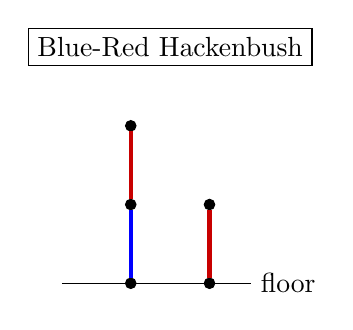
\begin{tikzpicture}
\node[draw] (title) at (1.5, 3) {Blue-Red Hackenbush};
\node (p1) at (0,0) {};
\node (p2) at (3,0) {floor};
\begin{scope} [every node/.style={scale=0.4, circle, draw, fill=black}]
	\node (p3) at (1,0) {};
	\node (p4) at (1,1) {};
	\node (p5) at (1,2) {};
	\node (p6) at (2,0) {};
	\node (p7) at (2,1) {};
	\draw (p1) -- (p2);
	\begin{scope} [ultra thick]
		\draw[blue] (p3) -- (p4);
		\draw[red] (p4) -- (p5);
		\draw[red] (p6) -- (p7);
	\end{scope}
\end{scope}
\end{tikzpicture}


In this game, a move is made by taking a single colored edge of the image and removing any edges that become disconnected from the floor. One player can only remove blue edges, and the other, red edges.

It is a common practice to assume that, unless specified otherwise, games will be played between the players \naming{Left (bLue)} and \naming{Right (Red)}.



% Theory
    \chapter{Theory}
    \textcolor{red}{This chapter should outline, compare and discuss key ideas, explanations, concepts, models and theories. You should present these ideas in a systematic, well-structured and logical sequence. It is expected that you use prominent and up-to-date books and articles. All literature should be referenced, not just for quotations, but also for ideas and information/knowledge drawn from the works of others.\\
Refer to the \href{http://libguides.lub.lu.se/plagiarism}{Teaching and Learning platform} for guidance on how to incorporate references into your text}

\section{Previous Research}
Lorem ipsum dolor sit amet, consectetur adipiscing elit. Duis ut ipsum nec orci interdum sollicitudin ut eu nunc. Pellentesque ultricies eros in justo sagittis, eget blandit velit aliquet. Aenean ac lectus nibh. Quisque ac est pellentesque, ullamcorper sem sit amet, pharetra quam. Morbi ullamcorper placerat diam, sed tincidunt odio.

\section{Theoretical Approach}
Lorem ipsum dolor sit amet, consectetur adipiscing elit. Duis ut ipsum nec orci interdum sollicitudin ut eu nunc. Pellentesque ultricies eros in justo sagittis, eget blandit velit aliquet. Aenean ac lectus nibh. Quisque ac est pellentesque, ullamcorper sem sit amet, pharetra quam. Morbi ullamcorper placerat diam, sed tincidunt odio.

    
% Data
    \chapter{Data}
    \input{sections/data}
    
% Methods
    \chapter{Methods}
    \input{sections/methods}
    
% Empirical Analysis
    \chapter{Empirical Analysis}
    \textcolor{red}{This chapter covers three areas: analysis of the data; discussion of the results of the analysis; and how your findings relate to the literature. The analysis of the data can be discussed here but the details of any analysis, such as statistical calculations, should be shown in the appendices. You should present any discussion clearly and logically and it should be relevant to your research questions/hypotheses or aims and objectives. Insert any tables or figures that you decide are important in a relevant part of the text not in the appendices, and discuss them fully. Make sure that you relate the findings of your primary research to your literature review. You can do this by comparison: discussing similarities and particularly differences. If you think your findings have confirmed some literature findings, say so and say why. If you think your findings are at variance with the literature, say so and say why.}
\section{Results}
Lorem ipsum dolor sit amet, consectetur adipiscing elit. Duis ut ipsum nec orci interdum sollicitudin ut eu nunc. Pellentesque ultricies eros in justo sagittis, eget blandit velit aliquet. Aenean ac lectus nibh. Quisque ac est pellentesque, ullamcorper sem sit amet, pharetra quam. Morbi ullamcorper placerat diam, sed tincidunt odio.

\textcolor{red}{When placing tables (\autoref{tab:econ}) within the body of the text, the citation is placed above the table.} 

\begin{table}[!ht]
  \centering
  {\small {\it \caption{The economic argument \label{tab:econ} \hcite{econ}}}}
  \includegraphics [scale=0.5]{images/the_economic_argument.png} \\
\end{table}

\vfill

\newpage 

\section{Discussion}
Lorem ipsum dolor sit amet, consectetur adipiscing elit. Duis ut ipsum nec orci interdum sollicitudin ut eu nunc. Pellentesque ultricies eros in justo sagittis, eget blandit velit aliquet. Aenean ac lectus nibh. Quisque ac est pellentesque, ullamcorper sem sit amet, pharetra quam. Morbi ullamcorper placerat diam, sed tincidunt odio.

\textcolor{red}{When placing figures (illustrations, pictures, graphs, diagrams, charts, maps etc.) within the body of the text, the citation is placed below the figure (\autoref{fig:moun})}

\begin{figure}[!h]
  \centering
  \includegraphics [scale=0.5]{images/dunning_kruger.png} \\
  {\small {\it \caption{Dunning–Kruger effect \label{fig:moun} \hcite{mount}}}}
\end{figure}
    
% Conclusion
    \chapter{Conclusion}
    \textcolor{red}{State the main conclusions of your study. State explicitly how and to what extent you have fulfilled your aims and objectives/answered your research questions/proved your hypotheses (whichever is appropriate). Your conclusions should follow logically from your findings and not contain any new material.}

\section{Research Aims}

\section{Research Objectives}

\section{Practical Implications}

\section{Future Research}

\section{Chapter Summary}

    
% Bibliography
    \phantomsection
    \addcontentsline{toc}{chapter}{References}%
    \bibliography{bibliography}
    
    \vspace{2.0cm}
    \textcolor{red}{Refer to \href{http://libguides.lub.lu.se/plagiarism}{LUSEM’s Harvard referencing guidelines} in the Teaching and Learning platform. \url{Lusem.lu.se/asks}}
    % The template provides \hcite and \mcite commands to present hyperlinked references in the 
    % Harvard referencing style '(Author, Year)'  and 'Author (Year)'
    % The template has an automated bibliography section based on references 
    % consistent with entries in the 'bibliography.bib' file 

% Appendices
    \appendix
    \chapter{(Appendix A title)}
    CGSuite, which stands for Combinatorial Game Suite, is a software suite used to study and research combinatorial games. The tool implements all the common methods in the field of study, which includes, but is not limited to, all the ones described in this text. CGSuite is widely used by people interested in Combinatorial Game Theory.

The package also includes a graphical interface and a interpreter, for its own scripting language, together with the game analysis functionality. CGSuite is open source software and the development is made on github and releases are published on sourceforge. The core functionality is implemented in Java and recent updates are also developed in scala. The maintainer of the project is Aaron Nathan Siegel, the autor of \textit{Combinatorial Game Theory} \cite{CGT}.

The typical use of the software is through the GUI and consists of manipulating small games, in the sense that results can be calculated in reasonable time, drawing them and their thermographs. CGSuite also allows users to extend the provided games and implement new games while still making use of the tools available. Extending the package is usually done using the same scripting language. 

The software is powerful enough to handle large cases sometimes, but in the cases such as evaluating a truly large instance or several large instances a personalized solution may be needed. Unfortunately there are no other complete implementations yet. There is ongoing development of another Surreal Numbers library, written in julia, but nothing that would replace a personalized solution.








    
     \chapter{(Appendix B title)}
    \input{sections/appendix_B}

\end{document}
%----------------------------------------------------------------------------------------------------%
